\subsection{Implementation}
We implement a framework in order  to simplify parameter estimation for 
pulse-chase RNA-seq experiments. 
We use \emph{R} programming environment, 
because it allows very flexible handling of user-specified models, 
includes implementations a variety of commonly used procedures and 
has powerfull plotting features \citep{rlang}.
\par A user need to provide
\begin{itemize}
 \item a count table with the raw read numbers
 \item a condition matrix (to infer sample fractions in the count table)
 \item formulas for the mean read numbers, e.g. 
 $r_\text{L}\sim \mu e^{-dt}$, (section~\ref{subsec:kinetics}).
\end{itemize}


\begin{figure}
 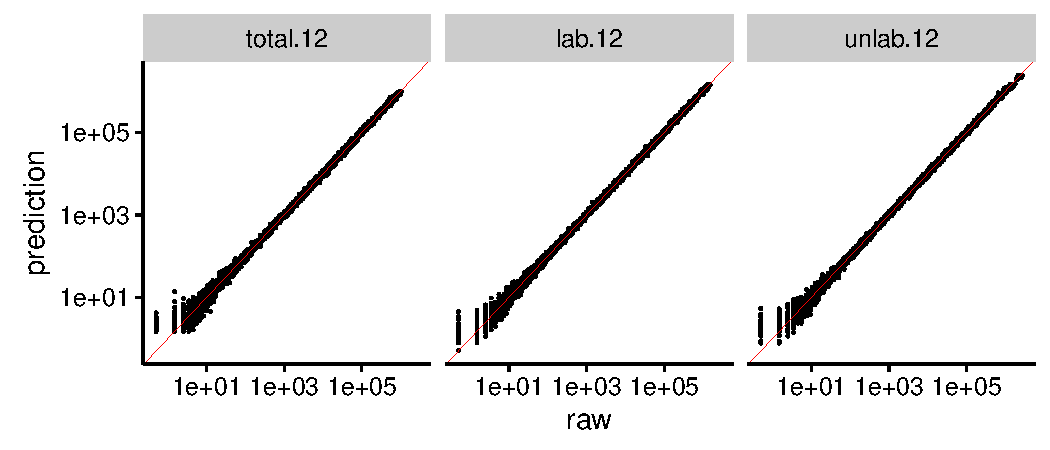
\includegraphics[width=\linewidth]{fig/predictions}
 \caption{Model predictions.}
\end{figure}

\begin{figure}
 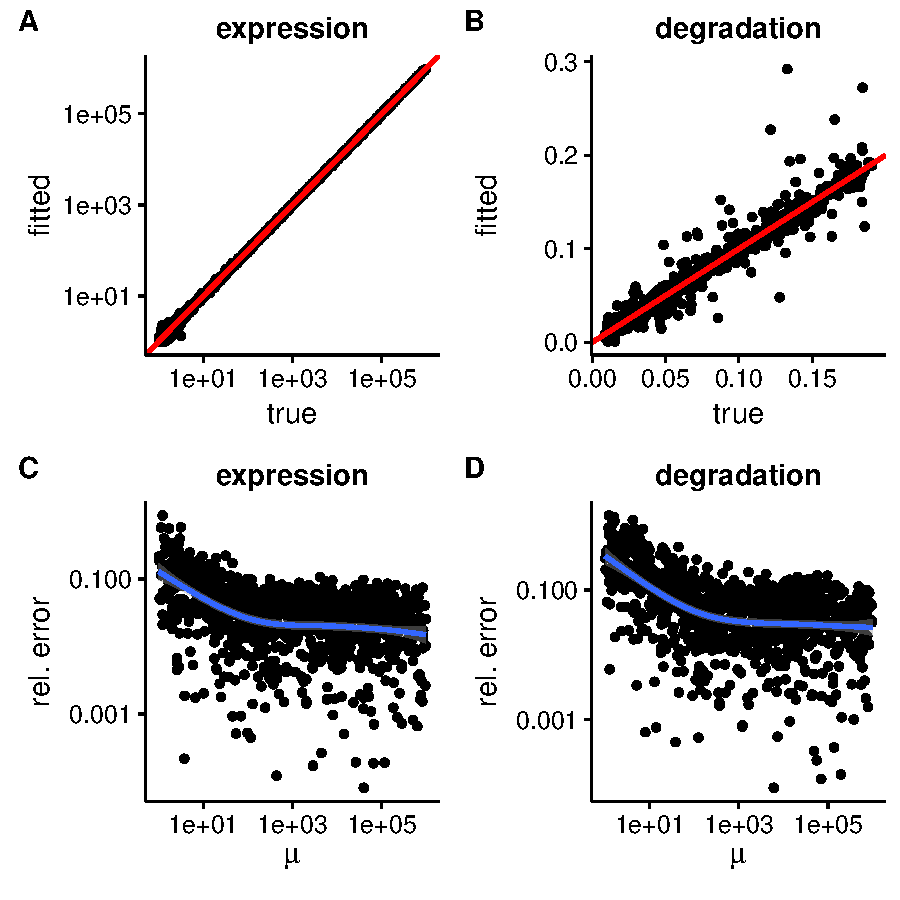
\includegraphics[width=\linewidth]{fig/parameters}\\
 \caption{Parameter misprediction.}
\end{figure}